
\chapter{Aufbau}


\thispagestyle{fancy}

\section{Photolumineszenzaufbau}
\begin{figure}[!htb]
    \centering
    \begin{minipage}[t]{\linewidth}
        \centering
        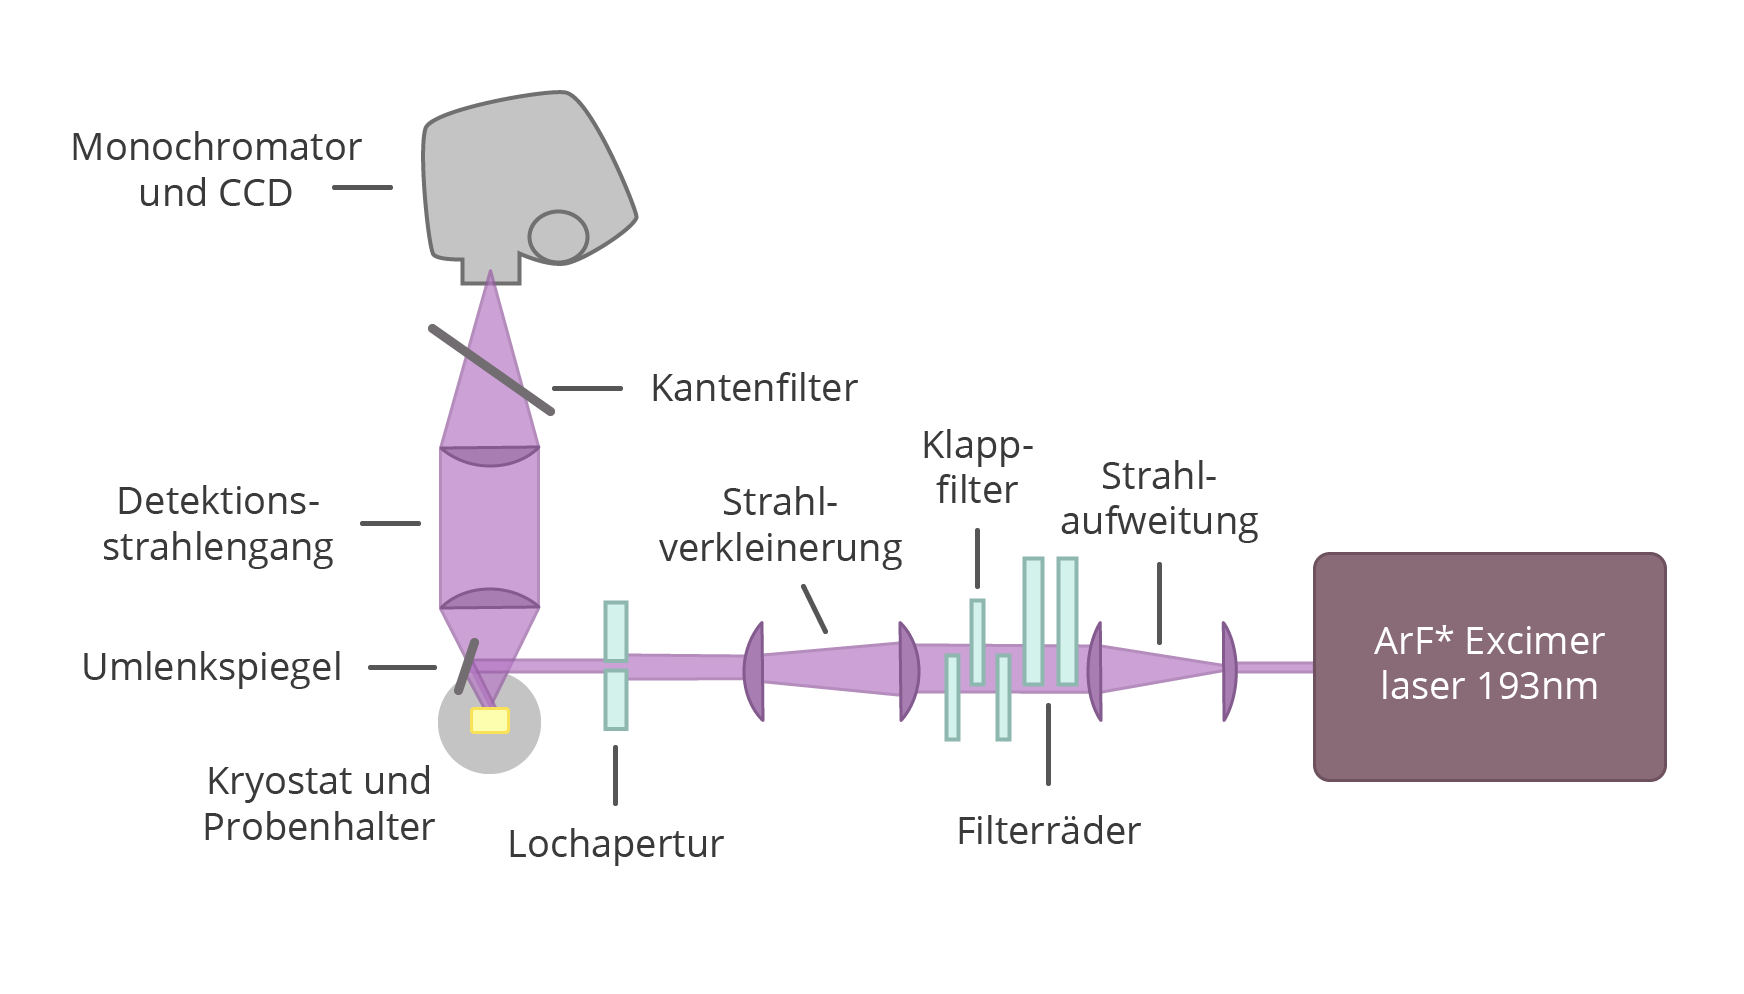
\includegraphics[width=0.8\linewidth]{Bilder/aufbauPL.png}
        \caption{Aufbau des Photolumineszenzmessplatzes der AG Kneissl. }
        \label{fig:wurtz}
    \end{minipage}% <- sonst wird hier ein Leerzeichen eingefügt
\end{figure}
\noindent
Für die experimentelle Untersuchung der UV-Photolumineszenz wurde der PL-Aufbau der AG-Kneissl, den Christoph Reich in der Zeit seiner Diplomarbeit aufgebaut und während seiner Promotion erweitert hat, verwendet~\cite{creich}. 
Als Anregungsquelle für die Photolumineszenz dient ein ArF-Excimerlaser mit einer Wellenlänge von $193 \ nm$ ($6,4 \ eV$). Mit dieser Wellenlänge ist er bestens geeignet für die Überbandanregung von Nitridhalbleitern. 
Des Weiteren bietet der Aufbau die Möglichkeit von temperaturabhängigen Untersuchungen von $5 \ K $ bis $300 K$. Dies ist auch die Grundlage für die Bestimmung der IQE. 
\newline
Der Laser mit dem Modellnamen "Xantos XS" von der Firma Coherent bietet eine maximale Emissionsenergie von $ 5 \ mJ $ und eine einstellbare Frequenz bis zu 500 Hz bei einer Pulsdauer von $5 \ ns$.
Durch interne Rückkopplung ist eine Energiestabilisierung möglich, die die Schwankung der Anregungsleistung auf 3 Prozent minimiert. 
\newline
Die Ansteuerung des kompletten Messvorgangs erfolgt durch die Messsoftware von Christoph Reich, entwickelt in der grafischen Programmiersprache "LabView" von Texas Instruments. Diese ermöglicht alle nötigen Einstellungen an Pumpen, Heizern, Laser, Filtern und Spektrometer, um einen nahezu komplett automatisierten Messvorgang zu starten. Spektren können so mit verschiedenen Parametern wie Position, Anregungsleistungsdichte, Temperatur, Energiebereich und Integrationszeit aufgenommen werden und auch ein Gaswechsel ist möglich.
\newline
Beginnend vom Laser wird im ersten Schritt der Laserstrahl durch ein Linsensystem, bestehend aus einer Zerstreuungs- und Sammellinse, aufgeweitet. Dieser Schritt ermöglicht es, die Anregungsleistungsdichte zu verringern, um die am Aufbau beteiligten Geräten, insbesondere die Filterräder, nicht mit zu hohen Leistungen zu beschädigen. Mit Hilfe der Filterräder ist es möglich, die Anregungsleistungsdichte 61 stufig zu variieren und somit leistungsdichteabhängige IQE Messungen zu machen. Als nächstes passiert der Strahl ein Linsensystem aus zwei Sammellinsen für eine Strahlverkleinerung. Vor dem Auftreffen des Strahles am Probenhalter im Kryostaten passiert der Strahl noch eine Lochblende. Sie dient der Entfernung achsennaher Strahlen und um bei Bedarf den Strahldurchmesser noch weiter zu verringern. 
\newline
Um den Strahl in Richtung des Probenhalters durch das Fenster im Kryostaten zu lenken, wird ein Spiegel mit einer dielektrischen Beschichtung benutzt. Der Laserstrahl durchdringt die Fenster des Kryostaten, welche speziell für eine hohe Transmission in diesem Wellenlängenbereich ausgelegt sind. Der Kryostat selbst ist horizontal und vertikal verschiebbar, um die Messung mehrerer Proben im Probenhalter in einem Messvorgang bei gleichen Bedingungen zu ermöglichen. Die Proben werden mit einem Kleber auf dem Probenhalter selbst befestigt, bevor dieser in den Kryostaten geschoben wird. 
Die Anregung der Proben mit dem Laserstrahl führt zur Proben spezifischen Emission von Licht. Diese wird von einer Linse im Strahlengang vor dem Detektor eingefangen und von einer zweiten Linse auf den Monochromatorspalt fokussiert.
\newline
Bei dem Monochromator handelt es sich um einen "`iHR 320"' des Herstellers "`Horiba"' . Zur Verfügung stehen drei Blazegitter mit $300 \thinspace \frac{Linien}{mm}$,
$600 \thinspace \frac{Linien}{mm}$ und $1800 \thinspace \frac{Linien}{mm}$. Bei der verwendeten Spaltbreite von $100 \thinspace \mu m$, entspricht die maximale Auflösung in etwa $5 \thinspace meV$ ($0,17 \thinspace nm$). Für Messungen oberhalb von $225 \thinspace nm$ besteht die Möglichkeit einen Kantenfilter in den Strahlengang zu stellen, mit dem das Laserstreulicht und dessen höhere Ordnungen aus dem Spektrum entfernt werden kann. Bei dem CCD Chip handelt es sich um das Modell "`Syncerity"' von "`Horiba"' der "`open electrode"' Bauart mit 1024x256 einzelnen Pixeln. 

\section{Messaufbau Lichtpolarisation}
\begin{figure}[!htb]
    \centering
    \begin{minipage}[t]{\linewidth}
        \centering
        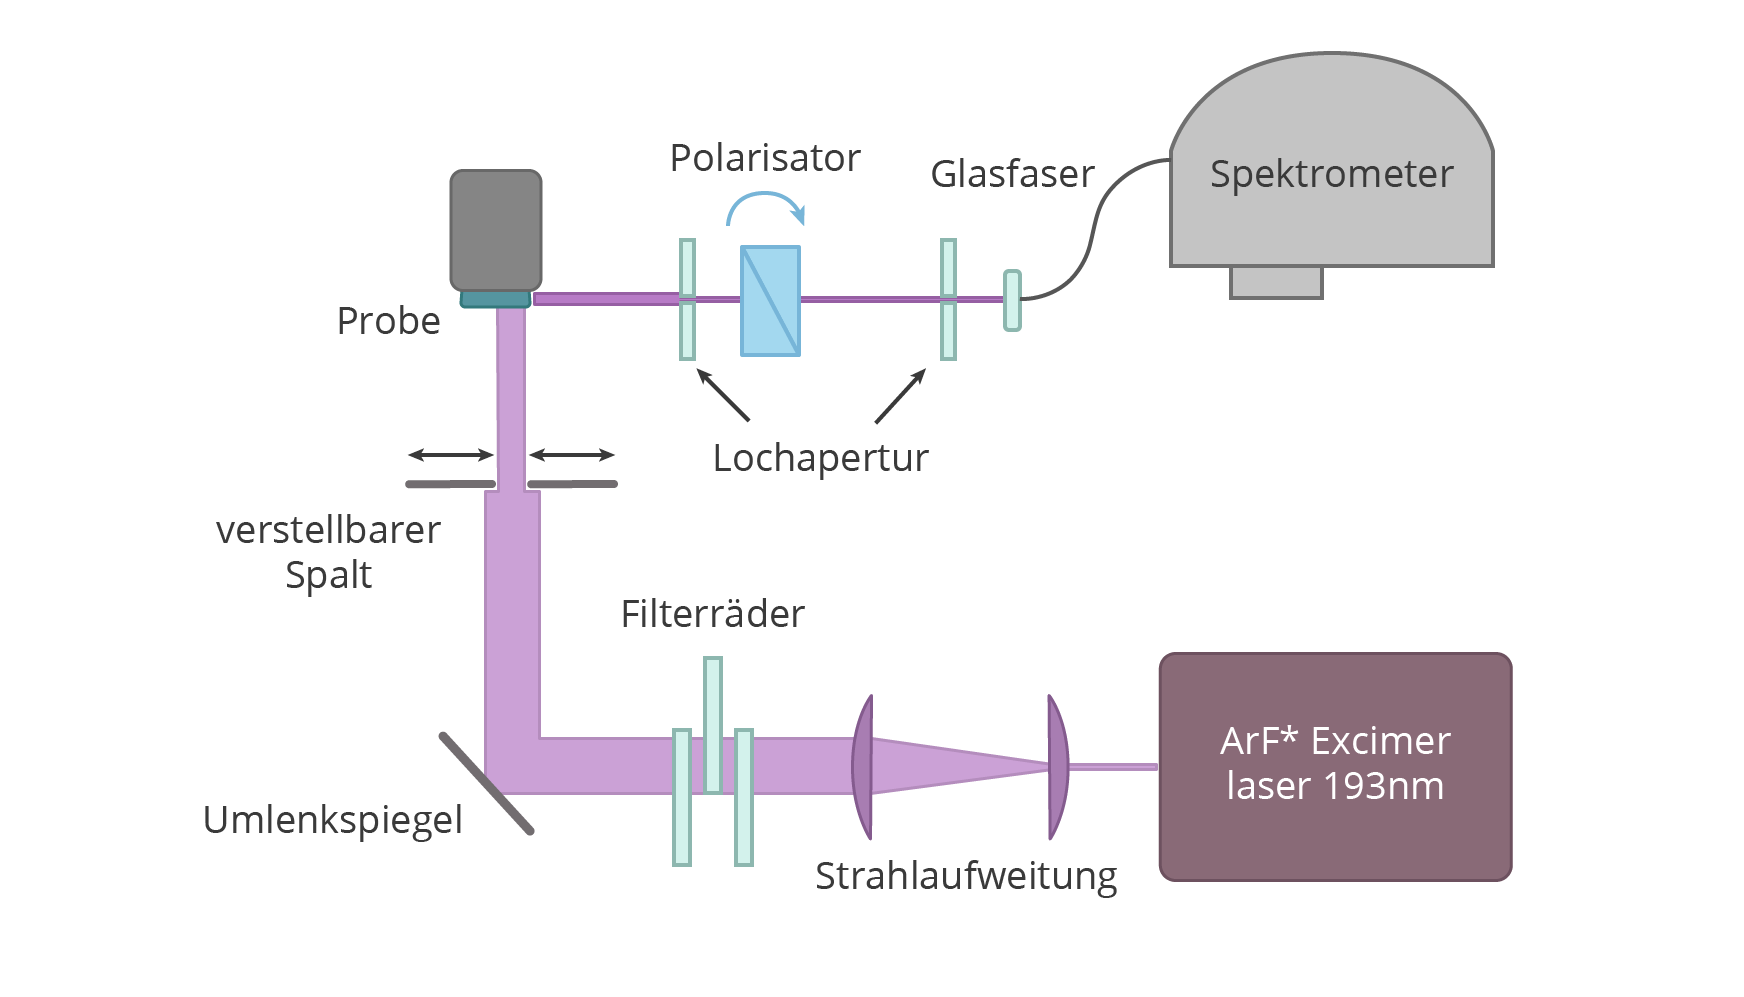
\includegraphics[width=0.8\linewidth]{Bilder/aufbauPol.png}
        \caption{Aufbau des Photolumineszenzmessplatzes der AG Kneissl zur Bestimmung der Polarisation. }
        \label{fig:wurtz}
    \end{minipage}% <- sonst wird hier ein Leerzeichen eingefügt
\end{figure}
\vspace{1cm}
\noindent
Für die Messung der Lichtpolarisation erfolgt die Anregung der untersuchten Proben senkrecht zur Oberfläche. Die Lumineszenz der Probe wird aus der Kante gemessen, weil TM-polarisiertes Licht nur vertikal zur c-Achse, wie in Abbildung \ref{fig:martintetm} sichtbar, emittiert wird. Die Lumineszenz wird dann unter kleinem Öffnungswinkel über eine Linse mit sich dahinter befindender Blende eingesammelt und parallelisiert. Das parallelisierte Licht wird dann durch einen Glan-Taylor-Polarisator geleitet. Dass das Licht parallelisiert ist, ist wegen der anisotropen Brechzahl des Polarisators wichtig. Diese ist neben der Polarisationsrichtung auch von dem Eintrittswinkel abhängig ist und entscheidet ob der Strahl transmittiert oder reflektiert wird \cite{0950-7671-25-12-304}. In Abhängigkeit der Orientierung des Polarisators wird TE- oder TM-polarisiertes Licht transmittiert und der eingestellte Winkel lässt sich $1\deg$ granular einstellen. 
